\chapter{BERT}

Das folgende Kapitel beschäftigt sich mit der Struktur der \textbf{B}idirectional \textbf{E}ncoder \textbf{R}epresentations from \textbf{T}ransformers. Wie aus dem Namen zu schließen ist, basiert BERT auf dem Transformer (\ref{Transformer}).

\section{Struktur von BERT} \label{BERT}

BERT basiert auf dem Transformer \cite{BERT:19}. Das BERT-Model nutzt die Hauptcharakteristik des Encoders, Beziehungen zwischen den Wörtern im Corpus zu erlernen. Im Vergleich zum Transformer, wo zwei Einheiten zusammenarbeiten, ist in BERT nur die Encoder-Einheit nötig, weil nur ein Sprachenmodel erstellt werden soll, wie beim Transformer werden die Eingaben vorverarbeitet. In dieser Hinsicht haben die beiden Modelle kleine Unterschiede. In BERT wird nicht nur Information über die Position der einzelnen Wörter eingelagert, sondern auch die Angaben über die Segmente der Eingabe (falls eine Eingabe aus mehreren Segmenten, bzw. Sätzen besteht) werden integriert. Außerdem werden diese im BERT-Model als Hyperparameter initialisiert. Das bedeutet, dass alle Positional- und Segmentvariablen erlernt werden müssen. Diese kleine Änderung erfordert ein unterschiedliches Vorgehen beim Lernen des Modells. Der Lernprozess von BERT wird aus diesem Grund in zwei Phasen aufgeteilt - Pre-training (erste Phase) und Fine-tuning (zweite Phase). Die erste Phase konzentriert sich auf die Erlernung der einzelnen Hyperparameter des Einbettungslayers. In dieser Phase soll die Token-Tabelle (Tokenizer) bereits verfügbar sein. Die zweite Phase des Lernens versucht, die vorgegebene Task zu lösen. Für das beste und schnellste Ergebnis sollte für die zweite Phase derselbe Tokenizer verwendet werden. Jedoch ist diese Anforderung kein Muss, denn die Anwendung von zwei getrennten Tabellen würde zu längeren Lernzeiten führen. Durch die große Anzahl an vortrainierten Modellen im Netz lohnt es sich, ein Modell wiederzuverwenden und für die eigene Task anzupassen. In den folgenden Kapiteln werden beide Phasen aufgeführt. Es wird zuerst der Prozess der Vorerlernung vorgestellt und danach wird erklärt, wie ein vortrainiertes Modell für die gewünschte Task angepasst werden kann.

\section{Implentierung} \label{BERT_Impl}

Die folgenden drei Kapitel stellen das BERT-Modell detaillierter vor und geben eine mögliche Implementierung des Modells mit der Bibliothek Tensorflow von Google. Die Implementierung basiert auf Publikationen \cite{BERT:19}, \cite{BERT_Pre:22} und \cite{BERT_Fine:22}. Im Paper \cite{BERT:19} aus dem 2019 wird ein neues Vorgehen im Bereich des Natural Language Processing vorgestellt. Die Autoren stellen eine bessere Alternative zur Fineeinstellung der Transformermodelle vor. Im Artikel wird die unidirektionale Beschränkung des Transformers verbessert, indem ein Masked-Language-Model (MLM) als Vortrainierungsziel verwendet wird. Das verwendete Modell maskiert zufälligerweise Tokens aus der Eingabe und die Idee ist, diese Token-IDs aus dem Kontext herzuleiten. Dieses Ziel verbindet den linken und rechten Kontext vom Satz und der trainierte Transformer ist bidirektional. Die Autoren kombinieren dieses Ziel mit dem Next-Sentence-Prediction-Ziel (NSP), sodass sie zwei Tasks gleichzeitig verarbeiten. Das Ziel der zweiten Aufgabe ist es vorauszusagen, ob zwei gegebene Sätze im Text nacheinander vorkommen.

In der zweiten Phase wird die Task nach Bedarf ausgesucht. Im vorliegenden Fall ist das eine Übersetzung aus dem Englischen ins Portugiesische. Die Task, die später gelöst werden soll, muss nicht vom Pre-Training abhängen. Das bedeutet, dass eine Zieländerung des vortrainierten Modells immer möglich ist, sobald ausreichend Daten vorhanden sind.

Als nächstes wird die Anpassung der Einbettungs- und Encoderparametern im Code vorgestellt.

\subsection{Pre-Training a BERT-Model}
Der Prozess des Vortrainierens erfordert die meiste Zeit von den beiden Phasen. Der Grund dafür ist die große Anzahl an Variablen im Modell. In der vorliegenden Ausarbeitung werden dieselben Mechanismen verwendet, die im Atrikel \cite{BERT:19} vorgestellt werden. Das heißt, dass zwei Tasks (NSP und MLM) gleichzeitig gelöst werden. Das Masked Language Model wurde im vorigen \cref{BERT_Impl} eingeleitet, aber in diesem Kapitel wird der Prozess näher vorgestellt. Die Eingabedaten werden speziell für das Modell vorbereitet. Laut dem Artikel \cite{BERT:19} werden 15\% der Wörter im Batch verborgen. Das bedeutet, dass höchstens 10 Wörter bei einer Größe des Batches von 64 und 5 Wörter bei einer Größe von 32 maskiert werden. Jedes Wort aus dem Batch hat eine gleich hohe Wahrscheinlichkeit von 10\% entweder maskiert oder durch ein weiteres Wort ersetzt zu werden. In 80\% der Fälle bleibt das Wort erhalten.

Beim Next-Sentence-Prediction ist die Aufgabe vorherzusagen, ob beide Sätze kontextuell verbunden sind. Hier werden in der Hälfte der Fälle zwei aufeinander folgende Sätze genommen. Die weiteren Paare sind zwei kontextuell unterschiedliche Sätze. In diesem Sinne gelten die eingebetteten Sätze als Input und haben einen Wert aus zwei Klassen als Label für die NSP-Task. Die Klassen können beliebig festgelegt werden, üblicherweise werden die Werte 0 (nicht benachbarte Sätze) und 1 (kontextuell benachbarten Sätze) verwendet. 

\subsection{Erstellen von Eingabe und Klasse}

Für das Vortrainieren wird das \textit{wikitext-2-v1} \cite{wikitext2:20} Corpus verwendet. Das Corpus ist eine Sammlung von Wiki-Artikeln in englischer Sprache. Außerdem besteht es aus mehr als 100 millionen Tokens. Die Trainingsdatei besteht aus mehr als 35 Tausend Zeilen Text. Der Datensatz ist im Literaturverzeichnis verlinkt und kann heruntergeladen werden. Als Erstes werden die Daten aus dem Corpus fürs Training vorbereitet.

Die Klasse Wiki2Corpus bereitet das ganze Corpus vor. Zuerst werden alle Wörter in Zahlen mit Hilfe eines Tokenizers verwandelt. Dafür wird aus der Bib-liothek \textit{d2l} \cite{d2l:21} der Tokenizer genutzt. Als nächstes wird die Vocabulary erstellt, damit Inferenzen des Modells später in Worte verwandelt werden. Der Wortschatz ergibt sich aus dem gesamten Text. Hier bietet d2l eine Vocabulary-Klasse, die jedem Wort aus dem Korpus einen Token zuweist. Die Klasse bietet die Möglichkeit auch seltene Wörter auszufiltern. Ein Programmcode, der diese Operationen darstellt, ist gegeben:

\begin{lstlisting}[language=Python, caption={Nutzung der Dive into Deep Learning (d2l) Bibliothek}]
paragraphs = [d2l.tokenize(paragraph, token='word') for paragraph in paragraphs]

self.vocab = d2l.Vocab(sentences, reserved_tokens=['<pad>', '<cls>', '<sep>', '<mask>'])
\end{lstlisting}

Als nächstes werden die Samples für das NSP-Model vorbereitet. In der utils.py Datei werden diese und zusätzlich nötige Methoden für die Vorbereitung erstellt. Diese sind gegeben:

\begin{lstlisting}[language=Python, caption={Erstellen der Trainingsdaten für NSP}]	
def get_nsp_data_from_paragraph(paragraph, paragraphs, max_len):
	nsp_data_from_paragraph = []
	for i in range(len(paragraph) - 1):
		# prepare sentence pairs and label
		sentence_a, sentence_b, is_next = _get_next_sentence(paragraph[i], paragraph[i + 1], paragraphs) 
		if len(sentence_a) + len(sentence_b) + 3 > max_len:
			continue
		token, segment = _get_tokens_and_segments(sentence_a, sentence_b) # add keywords
		nsp_data_from_paragraph.append((token, segment, is_next))
	return nsp_data_from_paragraph
\end{lstlisting}

Nachdem die Samples für das NSP-Model vorbereitet wurden, müssen die Eingaben und Labels für das MLM erzeugt werden. Die neu erzeugten Datensätze müssen mittels Schlüsselwörter abgegrenzt werden. Die Schlüsselwörter ['CLS'], ['SEP'], ['MASK'] und ['PAD'] müssen an die entsprechenden Positionen im Satz gefügt werden. Der ['CLS']-Token kennzeichnet den Beginn des Satzes. Der ['SEP']-Token wird am Ende des Satzes gestellt und so dient er auch zur Abgrenzung der Sätze, falls mehrere Sätze als Eingabe dem Model gegeben werden. Der Mask-Token ersetzt ein maskiertes Wort und der Padding-Token wird für die Erweiterung des Satzes bis zur maximalen Satzlänge verwendet. Die Einsetzung der Schlüsselwörter kann sowohl vor der Erstellung des Samples als auch nachher erfolgen. Die neu erzeugten NSP-Satzpaare werden für das MLM maskiert. Die Erstellung der Input und Labelpaare erfolgt wieder durch mehreren Methoden in utils.py:

\begin{lstlisting}[language=Python, caption={Erstellen von Trainingsdaten für MLM}]
def get_mlm_data_from_tokens(tokens, vocab):
	candidate_pred_positions = []
	for i, token in enumerate(tokens):
		if token in ['<cls>', '<sep>']:
			continue
		candidate_pred_positions.append(i)
	num_mlm_preds = max(1, round(len(tokens) * 0.15)) # number of masked tokens
	# Mask the sentences
	mlm_input_tokens, pred_positions_and_labels = _replace_mlm_tokens(tokens, candidate_pred_positions, num_mlm_preds, vocab)
	pred_positions_and_labels = sorted(pred_positions_and_labels, key=lambda x: x[0])
	pred_positions = [v[0] for v in pred_positions_and_labels]
	mlm_pred_labels = [v[1] for v in pred_positions_and_labels]
	# tokenize the sentences
	return vocab[mlm_input_tokens], pred_positions, vocab[mlm_pred_labels]
\end{lstlisting}

Am Ende sieht die generierte Datensammlung wie folgt aus:
\begin{lstlisting}[language=Python, caption={Eingabedaten}]
	 # input tokens    	 # segment vector	# sequence length # masked token index	  # weights for the label
	(self.all_token_ids, self.all_segments, self.valid_lens, self.all_pred_positions, self.all_mlm_weights,
	 # labels for the input # NSP labels for
	 self.all_mlm_labels, 	self.nsp_labels) = pad_bert_inputs(examples, max_len, self.vocab)
\end{lstlisting}

Die Vorbearbeitung ist nun abgeschlossen und die Trainingsdaten können verwendet werden. Der nächste Schritt ist die Erstellung des Modells. 
\subsubsection{BERT Class}\label{bert_class}
Die vorliegende Arbeit basiert auf dem im \cite{BERT:19} vorgestellten Modell. Für die gestellte Aufgabe werden folgende Hyperparameter definiert:

\begin{lstlisting}[language=Python,caption={Die Hyperparametern vom BERT}, label={lis:BERT_Base}] 	
cfg = {
	'batch_size': 64,
	'input_max_len': 64, # sequence length
	'num_layers': 12, # number of attention layers
	'd_model': 768,	# number of neurons im model
	'num_heads': 12, # number of heads in each attention layer
	'depth_FF_Layers': 1024 # number of feed forward neurons
}
\end{lstlisting}

Diese Konfiguration entspricht dem $BERT_{BASE}$-Modell, das im Artikel \cite{BERT:19} vorgestellt wird. Es wird zusätzlich das $BERT_{LARGE}$-Modell definiert, das durch folgende Werte charakterisiert wird: $num\_layer$ = 24,  $d_{model}$ = 1024, $num\_heads$ = 12. Das Base-Modell besitzt 110 Mio. Parameter, während das große Modell dreimal so viele Parameter aufweist - insgesammt 340 Mio. Dadurch ist das Trainieren eines BERT-Models sehr anspruchsvoll, jedoch empfiehlt es sich, auf ein vortrainiertes Modell zurückzugreifen, da auf diese Weise der Arbeitsaufwand um die Hälfte reduziert werden kann.

Das Modell wird in einer eigenen Klasse definiert. Die Bestandteile des BERT-Models werden als Programmcode gegeben:

\begin{lstlisting}[language=Python, caption={BERT-Struktur bei Pre-Training}]
self.encoding = BERTEncoderLayer(num_layers, d_model, num_heads, dff, input_vocab_length, maximum_positional_encoding, rate=rate, layer_norm_eps=layer_norm_eps)
self.nsp_layer = Dense(2)
self.mlm_layer = MLMLayer(input_vocab_length, d_model)
self.softmax = Softmax()
\end{lstlisting}

Das Modell besteht aus vier Schichten, zwei davon werden in separaten Klassen ausgelagert. Die zwei Klassen sehen wie folgt aus:

\begin{lstlisting}[language=Python, caption={Definition des BERT-Encoder-Layers}]
# BERTEncoderLayer.py
# The three embedding layers
self.embedding = Embedding(input_vocab_size, self.d_model)
self.segment_encoding = Embedding(2, self.d_model)
self.pos_encoding = tf.Variable(
initial_value=tf.random_normal_initializer(mean=1., stddev=initializer_range)(shape=[1, maximum_position_encoding, d_model]),
trainable=True)
self.dropout = Dropout(rate)
# The Transformer Encoder Layer: 12 heads and 12 Layers
self.encoder_layer = [EncoderLayer(self.d_model, num_heads, dff, rate, layer_norm_eps) for _ in range(self.num_layers)]
# MLMLayer.py
# A Sequential Fully Connected Model
self.mlp = Sequential()
self.mlp.add(Dense(num_hiddens, activation='relu'))
self.mlp.add(LayerNormalization())
self.mlp.add(Dense(vocab_size))
\end{lstlisting}

Die Einbettungsschicht besteht aus drei erlernbaren Unterschichten. Die Funktionalität der Schicht ist in der Abbildung \ref{embl} dargestellt:

\begin{figure}
	\centering
	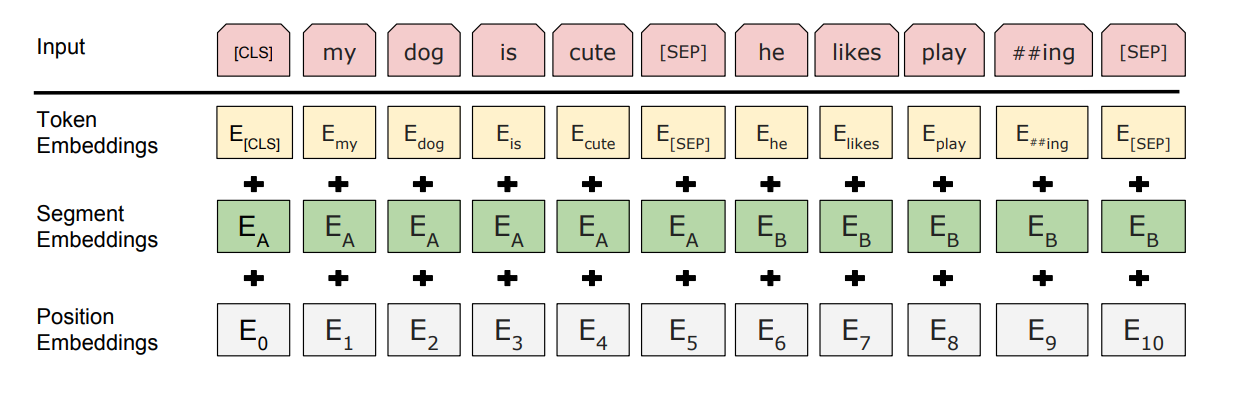
\includegraphics[scale=0.35]{images/bert_embedding_layer.png}
	\caption{BERT Eingabeschicht \cite{BERT:19}}
	\label{embl}
\end{figure}

Aus der Abbildung \ref{embl} kann man nicht nur die Funktion der Schichten lesen, sondern auch ihre Eingaben beobachten. In der Token-Embedding-Schicht werden die Tokens der Wörter gelesen und die Schicht liefert die zugehörige Vektor-Repräsentation. Die Segment-Embedding-Schicht erhält den Segmentenvektor, der bei der Vorverarbeitung der Eingabepaare erstellt wird. Der Positional-Embedding-Layer codiert die Wortindexen in Vektoren. Die Summe der Ergebnisvektoren aus den einzelnen Schichten liefert den eingebetteten Vektor, der die Eingabe im Encoder ist. 

\subsubsection{Optimizer und Loss-Funktion}\label{optimizer_and_loss}
Der nächste Schritt ist die Definition der Optimizer und die Fehlerfunktion. Für den vorliegenden Zweck wird der Adaptive-Movement-Optimizer verwendet. Laut \cite{CO:19} liefern Adam und RMSProp (\textbf{R}oot \textbf{M}ean \textbf{S}quare \textbf{Prop}agation) höhere Richtigkeit und niedrigere Fehlerrate als die anderen Optimizers, wie SGD(\textbf{S}tochastic \textbf{G}radient \textbf{D}escent) und AdaGrad(\textbf{Ada}ptiv \textbf{Gra}dients).  
Bei unserer ersten Task (Masked Language Processing) wird versucht, die maskierten Wörter zu bestimmen. Das impliziert, dass jedes maskierte Wort mehreren Klassen zugehören kann, bzw. aus vielen Wörtern bestehen kann. Aus diesem Grund können nur zwei Fehlerfunktionen verwendet werden, die \textit{CategoricalCrossEntropy} und \textit{SparseCategoricalCrossEntropy} sind.

\textit{CategoricalCrossentropy} ist geeignet, wenn die Ausgabe die partielle Zugehörig-keit zu den Klassen aufweist. Während dessen ist \textit{SparseCategoricalCrossentropy} besser geeignet, wenn die Ausgabe nur einen Integer-Wert beinhaltet bzw. daraus besteht. Dieser Integer stellt die zugehörige Klasse dar. Welche Fehlerfunktion verwendet wird, hängt nur von der Form der Ausgabe ab. Die vorliegende Arbeit beschäftigt sich überwiegend mit \textit{CategoricalCrossEntropy}, da die Ausgaben ein Softmax-Vektor sind. Später wird bei der Anpassung \ref{fine_tuning} wird \textit{SparseCategoricalCrossEntropy} verwendet.

\subsection{Fine-Tuning von einem BERT-Modell}\label{fine_tuning}

Das Modell für das Fine-Tuning wurde dem TensorflowHub \cite{tfhub:21} entnommen. Für diesen Zweck wird ein Modell mit den gleichen Hyperparametern, wie das im Unterkapitel \ref{bert_class} vorgestellte $BERT_{BASE}$ verwendet. Auf TensorflowHub stehen mehrere Modelle zur Wiederverwendung, hier unter anderem BERT-Multilangual-Cased-Modell, BERT-English-uncased, sowohl das Base-BERT-Modell als auch das Large-Modell. Dementsprechend kann das geeignete Modell für die Task ausgewählt werden. Im aktuellen Fall soll ein Translationsmodell aufgebaut werden. Für diesen Zweck wird das Multilingual-BERT-Modell \cite{BERTMM:21} genutzt. 

\subsubsection{BERT-Modell}

Das gelernte BERT-Modell kann wie folgt geladen werden:

\begin{lstlisting}[language=Python, caption={Laden von dem BERT-Modell}]
	# directly from the website
	pre_trained_model = 'https://tfhub.dev/tensorflow/bert_multi_cased_L-12_H-768_A-12/4'
	# or from file system
	pre_train_model_path = 'abs/path/to/Model/dir'
	encoder_input = hub.KerasLayer(pre_trained_model, trainable=True, name="BERT_Encoder")
\end{lstlisting}

Das Modell kann als eine Schicht geladen und somit in dem Modell angefügt werden. Für den Lernprozess braucht das Modell eine weitere Schicht, die die Prognose darstellen soll. Dafür bietet es sich an, eine einfache Dense-Schicht am Modell anzuhängen, die dann die Ausgabe des BERT-Modells mit einem Fully-Connected-Layer verbindet. Die Rolle der Dense-Schicht ist es, die Ausgabe in die richtige Shape zu verwandeln. Die Ausgabe vom BERT-Modell ist ein Vektor mit der Kardinalität \textit{batch\_size} $\times$ \textit{sequence\_length} $\times$ \textit{d\_model}. Die Dense-Schicht transformiert den Ausgabevektor in die Kardinalität \textit{batch\_size} $\times$ \textit{sequence\_length} $\times$ \textit{vocab\_size}. Die $sequence\_length$ entspricht der Länge des Satzes und jeder Index beschreibt ein Wort im Satz. Die Variable \textit{d\_model} repräsentiert die Anzahl der Eigenschaften, nach denen Wörter klassifiziert werden. Die Dense-Schicht verbindet somit die Eingeschaften der einzelnen Wörter zu einem Neuron, wobei die Ausgabe des Neurons ein Wert ist, der für oder gegen ein bestimmtes Wort aus dem Wortschatz spricht. Ein weiterer Schritt ist notwendig, damit diese Werte in Wahrscheinlichkeiten umgewandelt werden können, was nämlich durch die Anwendung der Softmax-Funktion erfolgt. Das heißt, dass das Modell aufgefordert wird, eine Prognose zu erstellen, wie die Übersetzung des Eingabesatzes lauten wird. Hier ist das Modell gegeben:

\begin{lstlisting}[language=Python, label=BERT_Definition, caption={Definition des BERT-Modells zur Anpassung}]
# input Layer with shape=(None, seq_length)
# these are the expected inputs in the BERT model
inputs = dict(
	input_word_ids=tf.keras.layers.Input(shape=(max_sentence_size,), dtype=tf.int32),
	input_mask=tf.keras.layers.Input(shape=(max_sentence_size,), dtype=tf.int32),
	input_type_ids=tf.keras.layers.Input(shape=(max_sentence_size,), dtype=tf.int32)
)
# BERT-Model
encoder_input = hub.KerasLayer(pre_trained_model, trainable=True, name="BERT_Encoder")
outputs = encoder_input(inputs)
net = outputs['sequence_output']
# dropout layer to help prevent overfitting
net = tf.keras.layers.Dropout(0.1)(net)
# dense layer for guessing
output = tf.keras.layers.Dense(vocab_size, activation=None)(net)
# This is our Model
model = tf.keras.Model(inputs, output)
\end{lstlisting}

\subsubsection{Datensatz}
Die Übersetzungstask ähnelt sehr einer Frage-Antwort-Task. Deswegen muss die Datensammlung im Voraus so vorbereitet werden, dass jeder Satz und seine Übersetzung gruppiert werden. Für diese Task wird der Datensatz $\textsc{\textit{/pt\_to\_en}}$ von der Datensatzsammlung $\textit{ted\_hrlr\_translate}$ verwendet. Der Datensatz ist über die Bibliothek $\textit{tensorflow\_datasets}$ zugänglich. Die Datensammlung enthält Sätze auf Englisch und Portugiesisch, also wird das Corpus für die Übersetzung aus dem Englischen ins Portugiesische genutzt. Die Datensammlung besteht jeweils aus 51785 Sätzen in Englisch und Portugiesisch, insgesamt also aus 103570 Sätzen. Die Sätze, die die erlaubte Sequenzlänge überschreiten, werden verworfen. Die ausgewählte Sequenzgröße beträgt 128 Wörter. Da die höhere Satzlänge eine längere Lernzeit bedeutet, wurden in Bezug auf die Hardware, die zur Verfügung steht, eine Sequenzlänge von 128 Wörtern, einschließlich Schlüsselwörter '[CLS]' und '[SEP]', ausgewählt. Das Laden der Datensammlung erfolgt über den folgenden Programmcode:

\begin{lstlisting}[language=Python, caption={Laden der Trainingsdaten}]
	model_name = 'ted_hrlr_translate_pt_en_converter'
	tf.keras.utils.get_file(f"{model_name}.zip", f"https://storage.googleapis.com/download.tensorflow.org/models/{model_name}.zip", cache_dir='.', cache_subdir='', extract=True)
	tokenizer = tf.saved_model.load(model_name)
\end{lstlisting}

Nach der Ausführung des Codes wird die Datensammlung im aktuellen Ordner heruntergeladen und entpackt. Mit Hilfe der dritten Zeile wird der Datensatz zur Nutzung geladen. Der nächste Schritt ist die Vorbereitung der Sätze für den Lernprozess. Hier müssen die Eingaben in einem Dictionary gespeichert werden, da das BERT-Modell so definiert wird. Wie die Eingabe aussieht, ist in der dritten Zeile aus dem Listing \ref{BERT_Definition} zu erkennen.

\subsubsection{Optimizer und Fehlerfunktion}

Als Nächstes werden die Optimizer und die Fehlerfunktion definiert. Für den Optimizer wird Adam verwendet, der über die üblichen Charakteristiken hinaus die Benutzung eines Schedulers für die Lernrate ermöglicht. Das bedeutet, dass die Rate im Laufe des Trainings angepasst werden kann. Die Konfiguration für den Optimizer ist durch den Programmcode gegeben:

\begin{lstlisting}[language=Python, caption={BERT Optimizer}, label=opt_loss]
	from official.nlp import optimization
	# learning rate
	init_lr = 5e-5
	# number steps pro epoch
	steps_per_epoch = len(train_input_array)
	# number of warmup steps
	num_warmup_steps = int(0.1 * steps_per_epoch)
	# the optimizer
	optimizer = optimization.create_optimizer(init_lr=init_lr,
	num_train_steps=steps_per_epoch,
	optimizer_type='adamw')
	# loss function
	tf.keras.losses.SparseCategoricalCrossentropy(from_logits=True)
\end{lstlisting}

Der Optimizer wird durch die Bibliothek \textit{official.nlp.optimization} bereitgestellt. Mit der Einstellung in dem \cref{opt_loss} wird der Optimizer konfiguriert, dass er für \textit{num\_warmup\_steps}-viele Iterationsschritte die Lernrate aufsteigen darf. Nach dem Ablauf der Schritten wird die Lernquote wieder gesunken.

Die genutzte Fehlerfunktion ist SparceCategoricalCrossEntropy. Der Grund dafür ist die Struktur des Labels und die Ausgabe des Modells (siehe Erklärung im Unterkapitel \ref{optimizer_and_loss}). Die Fehlerfunktion hat keine besondere Konfiguration, außer einen Parameter $\textit{from\_logits}$, der auf True gesetzt wird. Dadurch wird für die Fehlerfunktion im Voraus der Befehl vermittelt, dass keine Softmax-Funktion angewendet werden soll. Dementsprechend wird eine Sotfmax-Funktion zuerst ausgeführt, bevor die Fehlerrate errechnet wird.
